\chapter{System and conclusion}
\vspace{-5mm}
\section{System}
Successful integration of all of the components of the system was achieved in this design, where all of the implementations surpassed the design specifications. All of the transducer measurements were accurate for the full range specifications required in this design, and the system design was compatible with both $\SI{18}{VAC}$ and $\SI{24}{VAC}$ supply voltages. The GUI system implemented in this design was user friendly and included graphical representations of the load measurements, and as the purpose of this system was to be a smart power meter added functionality was added to calculate both the real and reactive power consumed by the load. The final system can be seen in Figure \ref{fig:PCB} with all of the functional subsystems indicated as per the colour scheme below, the full circuit schematic accompanying this design is shown in Figure \ref{fig:full_circuit_diagram}. 

\begin{figure}[ht]
    \centering
    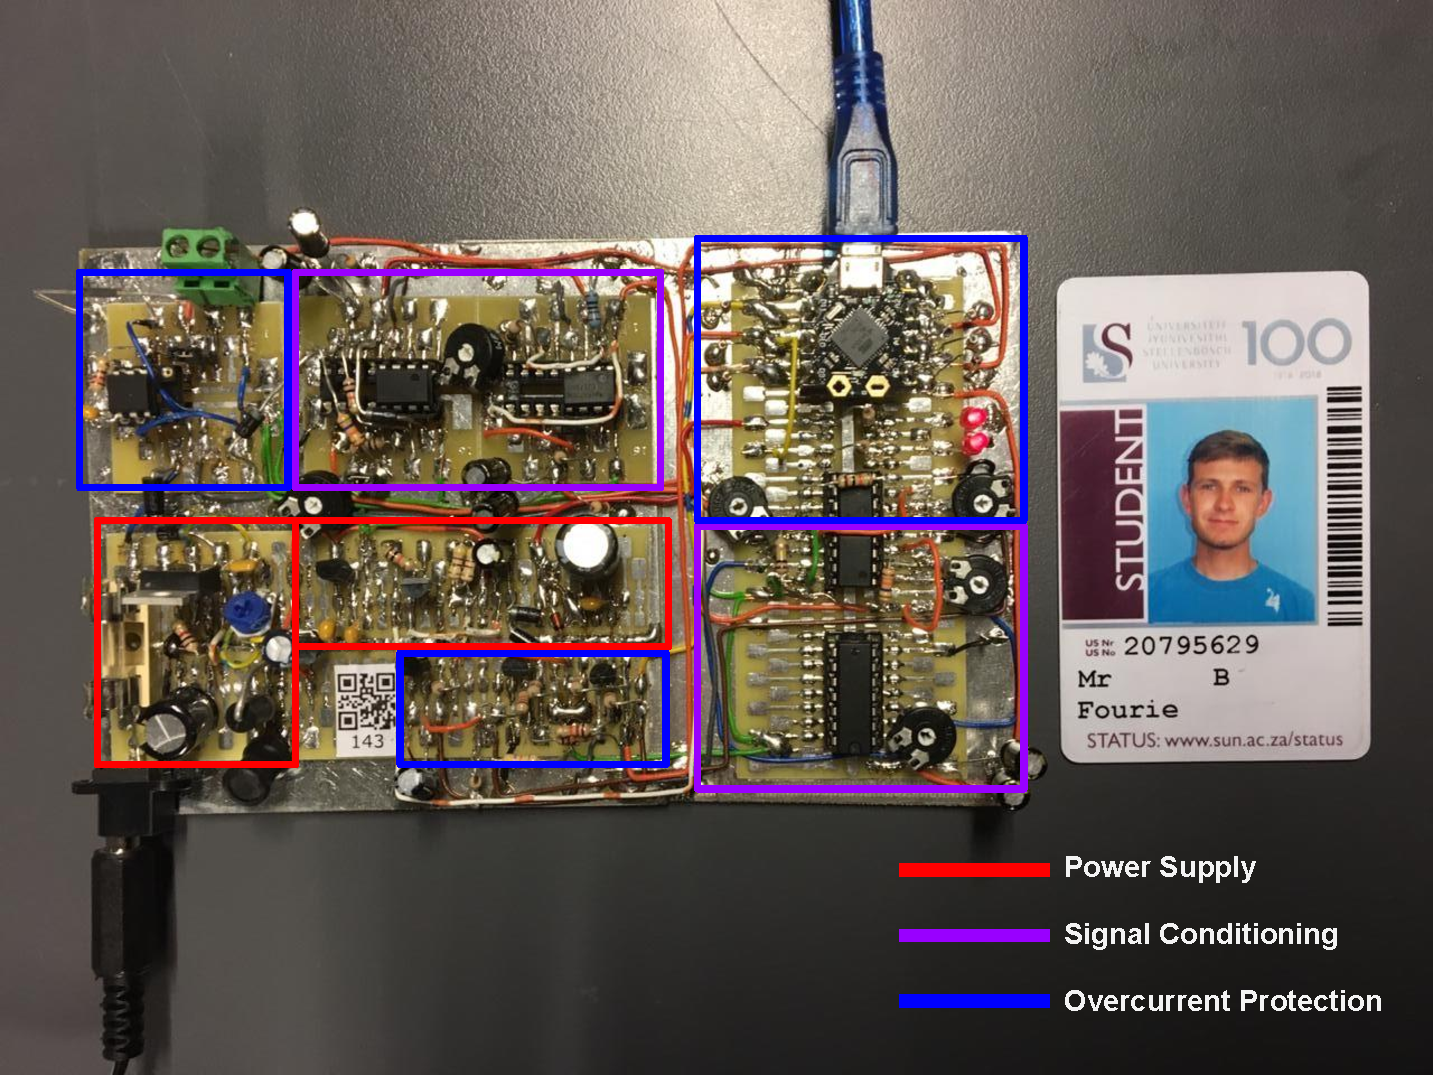
\includegraphics[width=0.8\linewidth]{./Figures/PCB.pdf}
    \caption{Complete PCB. } \label{fig:PCB}
\end{figure}

\section{Possible improvements}
Possible improvements to this design include implementing a true RMS calculation functionality to the smart power meter design.   In order to achieve this measurement samples for the voltage and current waveforms need to be taken every 20 milliseconds and all of these measurements need to be added to the respective arrays. Equations \ref{eq:truermsv} and \ref{eq:truermsi} can then be applied to these arrays to calculate a very accurate value for the RMS values.
\begin{align}
   V_{rms}&=\sqrt{\frac{\sum_{i=1}^{n} V_{i}^2}{n}} \label{eq:truermsv} \\
   I_{rms}&=\sqrt{\frac{\sum_{i=1}^{n} I_{i}^2}{n}} \label{eq:truermsi} 
\end{align}
Other further improvements that would contribute to the quality of this design would be adding storage capabilities for storing historic power usage. This data can be presented on the GUI as a summary of power used and could possibly assist a user in finding patterns in power usage and thus make decisions based on this information.

\section{Lessons learned}
The following is a list of life lessons learnt the hard way in the module E344:
\begin{itemize}
  \item Writing a report takes four times longer than you expect it to take.  
  \item There is no such thing as too many decoupling capacitors. 
  \item The best way to justify taking a break is by saying that you are running SPICE simulations. 
  \item Being clumsy with measuring probes can easily cause your circuit to go up in flames.
  \item A purely capacitive load will cause a short circuit in relatively high voltage AC circuits.
  \item Some students only realise they have a short circuit after they blow 10 fuses.
  \item Pretending to be busy is a good way of avoiding someone you have never met from asking for your components.
  \item Hilton is actually a really cool guy. 
\end{itemize}
